\documentclass[11pt]{report}
\usepackage[margin=1in]{geometry}
\usepackage[T1]{fontenc}
\usepackage{mathptmx}
\usepackage{amsmath,amssymb,booktabs,multirow,array,longtable,graphicx,siunitx,xcolor,microtype}
\usepackage[numbers,sort&compress]{natbib}
\usepackage{algorithm}
\usepackage[noend]{algpseudocode}
\usepackage[hidelinks]{hyperref}
\usepackage{caption}
\captionsetup{font=small,labelfont=bf}
\graphicspath{{../results/paper_figures/}}
\sisetup{group-separator={,},group-minimum-digits=4}
\makeatletter\newcommand{\tabinput}[1]{\@@input #1.tex }\makeatother
% Auto-generated by scripts/study/analyze.py -- do not edit.
\newcommand{\BanditMinusCspf}{50.8}
\newcommand{\BanditMinusCspfHi}{53.7}
\newcommand{\BanditMinusCspfLo}{47.1}
\newcommand{\BanditMinusGreedy}{21.2}
\newcommand{\BanditMinusGreedyHi}{24.1}
\newcommand{\BanditMinusGreedyLo}{17.6}
\newcommand{\BanditMinusMilp}{5.2}
\newcommand{\BanditMinusMilpHi}{8.1}
\newcommand{\BanditMinusMilpLo}{1.3}
\newcommand{\BanditMinusNoop}{120.7}
\newcommand{\BanditMinusNoopHi}{123.6}
\newcommand{\BanditMinusNoopLo}{117.0}
\newcommand{\BanditMinusOracleOne}{-29.2}
\newcommand{\BanditMinusOracleOneHi}{-23.7}
\newcommand{\BanditMinusOracleOneLo}{-36.1}
\newcommand{\BanditMinusRandom}{132.7}
\newcommand{\BanditMinusRandomHi}{136.1}
\newcommand{\BanditMinusRandomLo}{128.7}
\newcommand{\BanditMinusStatic}{121.7}
\newcommand{\BanditMinusStaticHi}{124.6}
\newcommand{\BanditMinusStaticLo}{118.0}
\newcommand{\BaselineReproCells}{21}
\newcommand{\BaselineReproMaxDiff}{3\cdot10^{-14}}
\newcommand{\Gap}{30.6}
\newcommand{\GapDeceptive}{14.6}
\newcommand{\GapDoublefailure}{-2.3}
\newcommand{\GapDz}{0.76}
\newcommand{\GapEveningpeak}{37.6}
\newcommand{\GapFinal}{39.1}
\newcommand{\GapFinalHi}{67.5}
\newcommand{\GapFinalLo}{3.5}
\newcommand{\GapFinalRootsPositive}{3}
\newcommand{\GapFlashcrowd}{23.6}
\newcommand{\GapFullday}{103.1}
\newcommand{\GapHi}{50.6}
\newcommand{\GapLinkfailure}{16.9}
\newcommand{\GapLo}{9.1}
\newcommand{\GapOverload}{20.3}
\newcommand{\GapRoots}{3}
\newcommand{\GapRootsPositive}{3}
\newcommand{\GapTHi}{82.8}
\newcommand{\GapTLo}{-21.7}
\newcommand{\GapWinRate}{86}
\newcommand{\HistBandit}{18.2}
\newcommand{\HistBanditRootA}{16.1}
\newcommand{\HistBanditRootB}{20.5}
\newcommand{\HistBanditRootC}{18.0}
\newcommand{\HistDeceptive}{-1.1}
\newcommand{\HistGap}{9.2}
\newcommand{\HistGapTHi}{17.3}
\newcommand{\HistGapTLo}{1.1}
\newcommand{\HistPPO}{9.0}
\newcommand{\HistPPORootA}{6.6}
\newcommand{\HistPPORootB}{8.3}
\newcommand{\HistPPORootC}{12.2}
\newcommand{\NDemands}{17}
\newcommand{\NDirLinks}{64}
\newcommand{\NLinks}{32}
\newcommand{\NRouters}{18}
\newcommand{\PPOMinusCspf}{19.2}
\newcommand{\PPOMinusCspfHi}{42.2}
\newcommand{\PPOMinusCspfLo}{3.4}
\newcommand{\PPOMinusGreedy}{-10.4}
\newcommand{\PPOMinusGreedyHi}{12.7}
\newcommand{\PPOMinusGreedyLo}{-26.2}
\newcommand{\PPOMinusMilp}{-34.1}
\newcommand{\PPOMinusMilpHi}{-7.8}
\newcommand{\PPOMinusMilpLo}{-55.7}
\newcommand{\PPOMinusNoop}{89.1}
\newcommand{\PPOMinusNoopHi}{112.1}
\newcommand{\PPOMinusNoopLo}{73.3}
\newcommand{\PPOMinusOracleOne}{-133.4}
\newcommand{\PPOMinusOracleOneHi}{-71.3}
\newcommand{\PPOMinusOracleOneLo}{-188.5}
\newcommand{\PPOMinusRandom}{101.1}
\newcommand{\PPOMinusRandomHi}{123.7}
\newcommand{\PPOMinusRandomLo}{85.5}
\newcommand{\PPOMinusStatic}{90.1}
\newcommand{\PPOMinusStaticHi}{113.1}
\newcommand{\PPOMinusStaticLo}{74.3}
\newcommand{\PeakOfferedGbps}{2.49}
\newcommand{\ReproBandit}{18.0}
\newcommand{\ReproBanditRootA}{14.7}
\newcommand{\ReproBanditRootB}{17.2}
\newcommand{\ReproBanditRootC}{22.2}
\newcommand{\ReproDeceptive}{14.7}
\newcommand{\ReproDeceptiveHi}{18.9}
\newcommand{\ReproDeceptiveLo}{10.6}
\newcommand{\ReproGap}{30.1}
\newcommand{\ReproGapHi}{50.8}
\newcommand{\ReproGapLo}{4.4}
\newcommand{\ReproMaxShiftBandit}{4}
\newcommand{\ReproMaxShiftPPO}{41}
\newcommand{\ReproPPO}{-12.0}
\newcommand{\ReproPPONeverPositive}{2}
\newcommand{\ReproPPORootA}{-20.1}
\newcommand{\ReproPPORootB}{13.0}
\newcommand{\ReproPPORootC}{-29.0}
\newcommand{\ReproRoots}{3}
\newcommand{\ReproRootsPositive}{3}
\newcommand{\SeqLiveAgreeH1}{100}
\newcommand{\SeqLiveAgreeH12}{46}
\newcommand{\SeqLiveAgreeH24}{34}
\newcommand{\SeqLiveAgreeH3}{73}
\newcommand{\SeqLiveAgreeH6}{56}
\newcommand{\SeqLiveCapturedH1}{100}
\newcommand{\SeqLiveCapturedH12}{59}
\newcommand{\SeqLiveCapturedH24}{52}
\newcommand{\SeqLiveCapturedH3}{78}
\newcommand{\SeqLiveCapturedH6}{61}
\newcommand{\SeqLiveSacrificeH1}{0}
\newcommand{\SeqLiveSacrificeH12}{45}
\newcommand{\SeqLiveSacrificeH24}{59}
\newcommand{\SeqLiveSacrificeH3}{19}
\newcommand{\SeqLiveSacrificeH6}{35}
\newcommand{\SeqLiveStates}{289}
\newcommand{\TestBandit}{25.2}
\newcommand{\TestBanditDecisionMs}{0.37}
\newcommand{\TestBanditDelivered}{95.31}
\newcommand{\TestBanditHi}{28.1}
\newcommand{\TestBanditLo}{21.5}
\newcommand{\TestBanditReroutes}{2.30}
\newcommand{\TestBanditRoots}{5}
\newcommand{\TestBanditSla}{164}
\newcommand{\TestCspf}{-25.6}
\newcommand{\TestCspfDecisionMs}{0.06}
\newcommand{\TestCspfDelivered}{93.64}
\newcommand{\TestCspfHi}{-23.2}
\newcommand{\TestCspfLo}{-28.0}
\newcommand{\TestCspfReroutes}{0.61}
\newcommand{\TestCspfRoots}{0}
\newcommand{\TestCspfSla}{243}
\newcommand{\TestGreedy}{4.0}
\newcommand{\TestGreedyDecisionMs}{0.06}
\newcommand{\TestGreedyDelivered}{94.85}
\newcommand{\TestGreedyHi}{6.3}
\newcommand{\TestGreedyLo}{1.7}
\newcommand{\TestGreedyReroutes}{4.60}
\newcommand{\TestGreedyRoots}{0}
\newcommand{\TestGreedySla}{187}
\newcommand{\TestMilp}{80.8}
\newcommand{\TestMilpDecisionMs}{637.23}
\newcommand{\TestMilpDelivered}{97.62}
\newcommand{\TestMilpHi}{83.4}
\newcommand{\TestMilpLo}{78.2}
\newcommand{\TestMilpReroutes}{5.68}
\newcommand{\TestMilpRoots}{0}
\newcommand{\TestMilpSla}{136}
\newcommand{\TestNoop}{-95.5}
\newcommand{\TestNoopDecisionMs}{0.00}
\newcommand{\TestNoopDelivered}{90.58}
\newcommand{\TestNoopHi}{-92.9}
\newcommand{\TestNoopLo}{-98.0}
\newcommand{\TestNoopReroutes}{0.00}
\newcommand{\TestNoopRoots}{0}
\newcommand{\TestNoopSla}{352}
\newcommand{\TestOracleOne}{372.3}
\newcommand{\TestOracleOneDecisionMs}{1649.99}
\newcommand{\TestOracleOneDelivered}{99.19}
\newcommand{\TestOracleOneHi}{380.8}
\newcommand{\TestOracleOneLo}{364.2}
\newcommand{\TestOracleOneReroutes}{1.07}
\newcommand{\TestOracleOneRoots}{0}
\newcommand{\TestOracleOneSla}{113}
\newcommand{\TestPPO}{-6.4}
\newcommand{\TestPPODecisionMs}{1.12}
\newcommand{\TestPPODelivered}{94.97}
\newcommand{\TestPPOHi}{16.6}
\newcommand{\TestPPOLo}{-22.2}
\newcommand{\TestPPOReroutes}{8.94}
\newcommand{\TestPPORoots}{3}
\newcommand{\TestPPOSla}{182}
\newcommand{\TestRandom}{-107.5}
\newcommand{\TestRandomDecisionMs}{0.02}
\newcommand{\TestRandomDelivered}{89.44}
\newcommand{\TestRandomHi}{-103.6}
\newcommand{\TestRandomLo}{-111.3}
\newcommand{\TestRandomReroutes}{11.66}
\newcommand{\TestRandomRoots}{0}
\newcommand{\TestRandomSla}{401}
\newcommand{\TestStatic}{-96.5}
\newcommand{\TestStaticDecisionMs}{0.01}
\newcommand{\TestStaticDelivered}{90.40}
\newcommand{\TestStaticHi}{-94.0}
\newcommand{\TestStaticLo}{-98.9}
\newcommand{\TestStaticReroutes}{0.37}
\newcommand{\TestStaticRoots}{0}
\newcommand{\TestStaticSla}{346}
\newcommand{\TotalCapacityGbps}{45.0}
\newcommand{\TpsBandit}{147}
\newcommand{\TpsPPO}{140}
\newcommand{\WallBandit}{45}
\newcommand{\WallPPO}{48}


\title{Persistent State Is Not Enough: When Incremental MPLS Traffic Engineering Needs Sequential Reinforcement Learning
\\[1ex]\large Technical report}
\author{Uğur Efe Yiğit}
\date{}

% The report reuses the paper's sections verbatim (so every number and claim
% is identical) and adds chapters with material that does not fit a paper.
% Paper-relative \input paths resolve through TEXINPUTS (see latexmkrc).

\begin{document}
\maketitle
\tableofcontents

\chapter*{Abstract}
\begin{abstract}
Reinforcement learning (RL) is increasingly applied to traffic engineering
(TE), but whether TE decisions are sequential enough to need it is rarely
measured. We study an incremental MPLS-TE problem in which routing state
persists, one label-switched path may move per five-minute interval, moves
are costly, a hold-down follows each move and an action mask enforces
failures and protected-class capacity---formally a Markov decision process.
On a flow-level 18-router backbone, a masked contextual bandit that predicts
only the immediate reward of each action beats MaskablePPO on all
\TestBanditRoots{} training roots (paired return difference \Gap{}, 95\,\% CI
[\GapLo, \GapHi]) and matches a non-learning per-interval min-max-utilization
MILP controller. The cause is the planning horizon, not the algorithm: PPO with
$\gamma=0$ matches the bandit, while PPO with $\gamma=0.995$ oscillates at
hold-down expiry and loses its network gains to reconfiguration costs, and a
bootstrapped value learner does not improve on the bandit. A clairvoyant
lookahead diagnostic explains why: with traffic held fixed, the
first-interval best action is the 24-interval best action in
\SeqFrozenAgreeHTwentyFour\,\% of states, against \SeqLiveAgreeHTwentyFour\,\%
under the true future, so almost all non-myopic value is anticipation of
exogenous change that the controller cannot observe. Delaying the effect of a
move by one interval reverses the ranking (PPO $-$ bandit $=\DelayPPOVs$
[\DelayPPOVsLo, \DelayPPOVsHi]). We also show that a prior internal study's
bandit result reproduces on different hardware while its PPO result does not.
Sequential RL for TE should be justified by measured temporal coupling, not by
the formal presence of state.
\end{abstract}


\chapter{Introduction}
\section{Introduction}
\label{sec:intro}

Traffic engineering (TE) decides which paths carry which traffic so that a
backbone delivers its demand without congestion, SLA violations or
needless reconfiguration. In MPLS networks the decision is concrete: each
traffic trunk rides one label-switched path, and an operator or controller
moves trunks between a few precomputed candidates as load
changes~\citep{rfc2702,rfc3209}. Because traffic varies over the day and
failures arrive unannounced, reinforcement learning (RL) is an appealing
tool, and deep RL has been applied to routing and TE in many
forms~\citep{valadarsky2017learning,xu2018drlte,zhang2020cfrrl,almasan2022drlgnn,bernardez2023magnneto}.

RL earns its machinery---value functions, discounting, credit assignment
over long horizons---only if today's decision changes tomorrow's options in
ways that a myopic decision rule would get wrong. Whether that is true of TE
is rarely measured. The strongest recent TE systems argue the opposite for
the standard setting, in which routing is re-optimized from scratch every
interval and therefore has no memory: Teal reduces its RL objective to a
one-step return~\citep{xu2023teal}, and DOTE reports that direct optimization
beats an RL-based scheme by a wide margin~\citep{perry2023dote}. Operational
MPLS-TE is different in exactly the property those arguments rely on. LSP
moves are incremental and signalled, controllers limit how many trunks change
at once, stability timers prevent a trunk from moving again too soon, and
protected traffic may move only where capacity is guaranteed. The current
assignment is then part of the state, a move constrains the future, and the
decision problem is a genuine Markov decision process.

This paper asks, for such a formulation, \emph{whether sequential RL is
needed, and why or why not}. We study a flow-level MPLS backbone (18 routers,
64 directed links, 17 demands with SLAs, four candidate LSPs each) in which a
controller may move one demand per five-minute interval, moves cost
reconfiguration effort, a three-interval hold-down follows each move, and an
action mask enforces failed links, hold-downs and protected-class capacity.
We compare MaskablePPO~\citep{schulman2017ppo,huang2022masking} with a masked
neural contextual bandit that regresses only the immediate reward of each
action, under identical observations, masks, budgets and paired traffic.

The comparison was first run as a governed study by the project that
developed the environment, which found the bandit ahead. We treat that study
as a claim to be tested. Our contributions are:

\begin{itemize}
\item \textbf{A reproduction and its lesson.} Retraining all of the closed
study's runs on different hardware with byte-identical training traffic, the
bandit's result reproduces and PPO's does not: floating-point differences
alone move PPO's per-root holdout return by up to \ReproMaxShiftPPO{} points
and the bandit's by at most \ReproMaxShiftBandit{} (\S\ref{sec:repro}).
\item \textbf{A controlled comparison with a non-learning optimizer.} On
\TestBanditRoots{} training roots and 140 disjoint test episodes the bandit
beats PPO on every root and is statistically indistinguishable from a
per-interval min-max-utilization MILP controller that does not learn at all
(\S\ref{sec:rq1}).
\item \textbf{A mechanism.} PPO's deficit is dominated by reconfiguration
cost: on most roots it settles into flipping a demand at every hold-down
expiry, a small immediate cost that its long-horizon advantage estimates fail
to attribute (\S\ref{sec:analysis}). Horizon and algorithm are separated by
varying the discount within each learner family (\S\ref{sec:rq2}).
\item \textbf{A measured sequentiality diagnostic.} Clairvoyant rollouts show
that the problem is far from myopic per decision under the true future, but
that almost all of the non-myopic value is anticipation of exogenous traffic
change; with traffic held fixed, the myopic choice is the 24-interval choice
in \SeqFrozenAgreeHTwentyFour\,\% of states (\SeqLiveAgreeHTwentyFour\,\% under the true future) (\S\ref{sec:sequentiality}).
\item \textbf{A regime where sequential RL is necessary.} Delaying the effect
of a move by one interval---a controlled form of actuation latency---removes
the bandit's signal by construction; the bandit collapses while PPO is
unaffected, reversing the ranking (\S\ref{sec:rq5}).
\end{itemize}

We make no algorithmic or theoretical claim. All code, configurations,
per-episode results and the scripts that produce every number, table and
figure in this paper are part of the artifact.


\chapter{Background and related work}
\section{Background and Related Work}
\label{sec:related}

\paragraph{MPLS traffic engineering.}
MPLS-TE steers traffic trunks onto explicitly routed label-switched paths
(LSPs)~\citep{rfc2702,awduche1999mpls}; RSVP-TE signals them and moves them with
make-before-break~\citep{rfc3209}, and the same ``choose one of a few candidate
paths'' primitive applies to segment-routing policies~\citep{rfc8402}.
Classical TE solves an optimization per traffic matrix---weight
setting~\citep{fortz2000ospf}, oblivious and semi-oblivious
routing~\citep{applegate2003oblivious,kumar2018smore}, robust
TE~\citep{wang2006cope}, multicommodity-flow formulations minimizing the maximum
link utilization~\citep{wang2008overview}---or adapts online across a fixed set
of paths~\citep{elwalid2001mate,kandula2005texcp}. Production SDN WANs re-solve
periodically~\citep{jain2013b4,hong2013swan}. TeXCP~\citep{kandula2005texcp}
made the point that online TE must be stable as well as responsive, which is
why our formulation prices moves and imposes a hold-down.

\paragraph{Learning for routing and TE.}
RL for routing dates to Q-routing~\citep{boyan1993qrouting}. Deep RL has been
applied to intradomain routing~\citep{valadarsky2017learning,stampa2017drl},
utility-maximizing TE~\citep{xu2018drlte}, critical-flow
rerouting~\citep{zhang2020cfrrl,pei2024efficientte}, GNN-based and multi-agent
TE~\citep{almasan2022drlgnn,hope2021gddr,bernardez2021ml,bernardez2023magnneto,geng2020marlte,gui2024redte}.
The strongest recent systems, however, are not sequential: Teal argues that a
TE allocation for one interval does not affect future intervals and reduces
the RL return to one step~\citep{xu2023teal}; DOTE trains a network end to end
on the realized utilization and reports that an RL-based scheme is markedly
worse~\citep{perry2023dote}; FIGRET and HARP are one-shot learned
TE~\citep{liu2024figret,alqiam2024harp}. Several DRL-TE formulations are, in our
reading, contextual bandits in disguise: the state is the exogenous traffic
history and actions do not influence it~\citep{valadarsky2017learning,zhang2020cfrrl}.
Our setting differs in the property those arguments rely on: the routing
configuration persists, changes are incremental (one LSP per interval), costly
and subject to hold-down, so the current assignment is endogenous state.

\paragraph{When simple methods win.}
Deep-RL results are sensitive to implementation and tuning and need careful
statistics~\citep{henderson2018matters,engstrom2020implementation,andrychowicz2021matters,agarwal2021precipice,patterson2024empirical};
random search matches model-free deep RL on standard control
tasks~\citep{mania2018random}; in networking, a year-long randomized trial found
that learned bitrate control did not beat a simple buffer-based
rule~\citep{yan2020puffer}, and a re-examination of RL for optical resource
allocation found that improved heuristics match or beat the published
agents~\citep{doherty2025hype}. Our contribution is not another instance of
this pattern but a controlled attribution of it to horizon versus algorithm.

\paragraph{Contextual bandits and horizon.}
A regression oracle on immediate rewards with simple exploration is a standard
contextual-bandit design~\citep{langford2007epoch,foster2020beyond}, and greedy
methods are competitive when contexts are diverse~\citep{bietti2021bakeoff}.
Theory shows that long horizons need not make RL much harder than bandits in
sample complexity~\citep{zhang2021rlbandits}, while a planning horizon or
discount shorter than the true one can improve learned policies with limited
data~\citep{jiang2015horizon,petrik2008biasing,amit2020discount}. Laidlaw et
al.\ define the \emph{effective horizon}, the lookahead depth needed to find the
optimal action when leaves are evaluated by a base policy, and show it predicts
deep-RL success~\citep{laidlaw2023effective,laidlaw2024stochastic}. Congested
bandits formalize rewards that depend on recent actions over a short
window~\citep{awasthi2022congested}. Potential-based
shaping~\citep{ng1999shaping} is policy-invariant only for the discount it is
defined with---a caveat for any $\gamma=0$ learner trained on a shaped reward.
To our knowledge no TE study measures the sequentiality of its decision problem
or separates horizon from algorithm in a learner comparison.

\paragraph{Action masking.}
Masking invalid actions in policy-gradient methods is theoretically justified
and practically important when many actions are illegal~\citep{huang2022masking}.
Masks are a form of safe exploration with external knowledge~\citep{garcia2015safe};
constrained MDPs~\citep{altman1999cmdp,achiam2017cpo} are the alternative we do
not pursue. Flow-level simulation may not transfer to packet
dynamics~\citep{boltres2024packerl}; we return to this in
Section~\ref{sec:limitations}.


\chapter{Problem formulation}
\section{Problem Formulation}
\label{sec:formulation}

We state the decision problem exactly as implemented (Environment~V2 of the
artifact, frozen at commit \texttt{dca533b}); Appendix~\ref{app:formulation}
gives every constant.

\paragraph{Network and demands.}
The backbone is a directed graph $G=(V,E)$ with $|V|=18$ routers (four ingress
and four egress provider-edge routers, eight core and two aggregation routers)
and $|E|=64$ directed links (32 bidirectional links, \SIrange{250}{2000}{Mb/s}
per direction; Fig.~\ref{fig:topology}). There are $|\mathcal D|=17$ demands in
six classes, each with a priority $\pi_d\in\{1,\dots,6\}$, a delay and a loss
SLA, and a \emph{protected} flag (voice and critical traffic). Each demand
has a fixed, ordered set of $k=4$ candidate label-switched paths
$\mathcal P_d=(p_{d,0},\dots,p_{d,3})$, computed once by Yen's algorithm under
role, hop-count and propagation-delay constraints; $p_{d,0}$ is the
administratively shortest valid path.

\paragraph{Exogenous traffic.}
The offered rate of demand $d$ is
$v_d(t)=b_d\,f_{\kappa(d)}(h(t))\,m\,\eta_d(t)\,\mathrm{clip}(1+n_d(t),0.4,2)$:
a class-specific diurnal profile, a scenario multiplier, scripted or randomized
burst / flash-crowd factors and per-demand AR(1) noise
($n_d(t)=0.9\,n_d(t-1)+\sigma_d\varepsilon$, one step per simulated minute).
Link failures and recoveries are scripted or randomized events. Nothing in the
exogenous process $\xi_t$ depends on routing, which makes comparisons between
controllers exactly paired.

\paragraph{State and transitions.}
The controllable state $y_t$ holds, for each demand, its current candidate
$x_d$, a disconnection flag, the remaining \emph{dwell} (hold-down) $\omega_d$,
the previous traffic-engineering (TE) path and its age. The Markov state is
$s_t=(y_t,\xi_t)$. Decisions are taken every \SI{5}{min}; an interval is
simulated as five one-minute ticks in which a damped fixed-point solver
computes carried flow, per-link loss
($0$ below 90\,\% utilization, quadratic to 2\,\% at 100\,\%, $1-0.98/\rho$
above), M/M/1-shaped queueing delay and per-demand SLA status. A link failure
triggers immediate, free fast-reroute of the affected demands to their
cheapest live candidate. Because $\xi$ is action-independent,
\begin{equation}
P(s_{t+1}\mid s_t,a_t)=P_\xi(\xi_{t+1}\mid\xi_t)\;
\mathbb 1\!\left[y_{t+1}=\Psi(y_t,a_t,\xi_{t:t+1})\right],
\label{eq:transition}
\end{equation}
so an action influences the future \emph{only} through the routing state,
which persists until changed.

\paragraph{Actions and masks.}
$\mathcal A=\{0\}\cup\{(d,p)\}$, $|\mathcal A|=69$: action $0$ changes nothing;
$(d,p)$ moves demand $d$ to candidate $p$. At most one TE change is made per
interval. The legality mask is
\begin{equation}
m_t(d,p)=\mathbb 1[\text{$p_{d,p}$ is up}]\,\mathbb 1[p\neq x_d]\,
\mathbb 1[\omega_d=0]\,
\mathbb 1\!\left[\neg\mathrm{prot}_d\ \vee\ \max_{e\in p_{d,p}}\hat G_e/c_e\le1\right],
\label{eq:mask}
\end{equation}
with $m_t(0)=1$, where $\hat G_e$ is the projected gross load on link $e$ after
the move. An accepted move starts a three-interval dwell. The last factor
couples demands: where one demand is routed changes which moves are legal for
protected demands.

\paragraph{Reward.}
With $\mathrm{DR}$ the delivered ratio, PD/UD the priority-weighted protected
and unprotected disconnected fractions, SEV a bounded priority-weighted SLA
severity, $\rho^{\max}$ the worst link utilization and OV the overload ratio,
\begin{equation}
r_t=\underbrace{2\mathrm{DR}-30\mathrm{PD}-8\mathrm{UD}-6\mathrm{SEV}
-2g(\rho^{\max})-6\mathrm{OV}}_{U_t}
+0.2\big(0.995\,\Phi_{t+1}-\Phi_t\big)-C^{\mathrm{TE}}_t-0.05\,\mathbb 1[\text{rejected}],
\label{eq:reward}
\end{equation}
where $g(\rho)=\log(1+\max(0,(\rho-0.7)/0.3))$, $\Phi=\tanh(U/10)$ evaluated at
interval boundaries, and the move cost
$C^{\mathrm{TE}}=0.08+0.30\,\mathrm{vol}+0.12\,\mathrm{div}+0.30\,\mathrm{rev}$
charges the moved traffic share, the edge-set divergence between old and new
path and returns to the previous path within six intervals. The reward is the
exact sum of twelve logged components.

\paragraph{What kind of problem is this?}
With respect to $s_t$ the problem is a finite-horizon MDP with state-dependent
action sets: routes persist, moves lock a demand for three intervals, reversal
costs depend on history, and the protected-class mask couples demands. The
learners observe $o_t\in[0,1]^{604}$, which contains the routing state (current
and previous path, dwell, path age), per-link utilization, per-demand health
relative to SLA, and the projected bottleneck of every candidate move, but not
the clock, the noise state or future events; with respect to $\xi$ the problem
is therefore partially observable. A contextual bandit that regresses
$\mathbb E[r_t\mid o_t,a_t]$ discards the persistence of a new configuration
beyond the first interval, the opportunity cost of the dwell lock, future
reversal costs and the effect on other demands' legal sets. It keeps the first
interval of a move's effect because, in the frozen environment, a move carries
traffic in the interval in which it is made. Section~\ref{sec:sequentiality}
measures how much the discarded terms matter.

\section{Environment details}
\label{app:formulation}

All values are generated from the configuration files by
\texttt{scripts/study/analyze.py}. The topology has \NRouters{} routers,
\NLinks{} bidirectional links (\NDirLinks{} directed), \TotalCapacityGbps{}\,Gb/s
of total directed capacity, and \NDemands{} demands whose base (profile-peak)
rates sum to \PeakOfferedGbps{}\,Gb/s.

\begin{table}[h]
\centering\small
\caption{Traffic classes. Priority weights $q_d=\pi_d/6$ enter the SLA and
disconnection terms; protected classes may only be moved onto candidates whose
projected gross bottleneck utilization is at most 100\,\%.}
\label{tab:classes}
\begin{tabular}{@{}lrrrlll@{}}
\toprule
Class & Priority & Delay SLA (ms) & Loss SLA (\%) & Protected & Profile & Demands \\
\midrule
\input{tables/env_classes}
\bottomrule
\end{tabular}
\end{table}

\begin{table}[h]
\centering\small
\caption{Scenarios. Learners train only on \texttt{random\_day}, whose bursts,
single link failure (probability 0.5) and flash crowd (probability 0.3) are
drawn per episode; all seven evaluation scenarios are scripted and differ from
the training distribution.}
\label{tab:scenarios}
\begin{tabular}{@{}lrrrrl@{}}
\toprule
Scenario & Start (h) & Decisions & Multiplier & Noise $\sigma$ & Events \\
\midrule
\input{tables/env_scenarios}
\bottomrule
\end{tabular}
\end{table}

\paragraph{Observation (604 features, feature-major, all in $[0,1]$).}
Per directed link: $\mathrm{sat}(\rho_e)=\rho_e/(1+\rho_e)$ and the up flag
($2\times64$). Per demand ($28\times17$): $\mathrm{sat}$(offered/base), priority$/6$,
protected flag, $\mathrm{sat}$(delay/SLA), $\mathrm{sat}$(loss/SLA), path age$/12$
(capped), dwell$/3$, disconnected flag, one-hot current path (4), one-hot
previous TE path (4), candidate liveness (4), candidate propagation delay$/100$\,ms
(4), and $\mathrm{sat}$ of the projected gross bottleneck utilization of moving
to each candidate (4). Time of day, episode progress and future events are
deliberately excluded.

\paragraph{Episode boundaries.} Events scheduled at minute $t$ are applied in the
right-closed window $(t-1,t]$, so the observation at a boundary reflects every
event up to that time. Episodes never terminate; they are truncated at the
scenario end, so paired controllers have identical horizons.


\chapter{Methods}
\section{Methods}
\label{sec:methods}

All learners see the same observation and the same authoritative mask, train
on the same randomized scenario for the same number of environment
transitions, and are evaluated deterministically (masked argmax).

\paragraph{MaskablePPO.}
We use the \texttt{sb3-contrib} implementation~\citep{raffin2021sb3} with
invalid-action masking~\citep{huang2022masking}: logits of illegal actions are
set to $-10^{8}$, so $\pi_\theta(a\mid o,m)\propto m(a)e^{z_\theta(o)_a}$, and the
same mask is applied in rollouts, gradient steps and inference. Advantages use
GAE~\citep{schulman2016gae} and the clipped surrogate
objective~\citep{schulman2017ppo} with value and entropy terms. The study's
default configuration (inherited unchanged from the closed study) is
$\gamma=0.995$, $\lambda=0.95$, learning rate $3\cdot10^{-4}$, 16 environments
$\times$ 512 steps per rollout, batch 512, 8 epochs, clip $0.2$, entropy
$0.01$, separate $[256,256]$ tanh networks.

\paragraph{Masked neural contextual bandit.}
A $604$--$256$--$256$--$69$ ReLU network $\hat r_\theta(o,\cdot)$ predicts the
immediate reward of every action. Actions are chosen by masked
$\varepsilon$-greedy ($\varepsilon$ linear from $0.2$ to $0.02$ over $2\cdot10^5$
transitions; random actions are drawn from the legal set). A replay buffer of
the last $10^5$ tuples $(o,a,m,r)$ is sampled every 64 transitions for one
Adam step on the Huber loss between the \emph{selected} head and the observed
reward. There is no next state, discount, target network or bootstrapping.
At 400k transitions the bandit performs 6{,}187 gradient steps, PPO 6{,}144.

\paragraph{Masked Q-learner with discount $\gamma$.}
To vary the planning horizon \emph{without changing anything else}, we extend
the bandit by a single parameter. For $\gamma>0$ the regression target becomes
the normalized double-DQN~\citep{mnih2015dqn} target
\begin{equation}
y=(1-\gamma)\,r+\gamma\,Q_{\bar\theta}\big(o',\textstyle\arg\max_{a':m'(a')=1}Q_\theta(o',a')\big),
\label{eq:qtarget}
\end{equation}
with a target network copied every 250 updates; the maximization is over legal
successor actions only. The factor $(1-\gamma)$ rescales all action values of
one $\gamma$ by a common constant and leaves the greedy policy unchanged; it
keeps the Huber transition point comparable across $\gamma$. With $\gamma=0$
the learner is the bandit, bit for bit (unit-tested).

\begin{algorithm}[t]
\caption{Masked value learner (bandit for $\gamma=0$). Source:
\texttt{experiments/masked\_bandit.py}, \texttt{study/learners.py}.}
\label{alg:value}
\small
\begin{algorithmic}[1]
\State observe $o$ from 16 environments
\For{each vector step}
  \State $m\gets$ masks; $a\gets\arg\max_{a:m(a)=1}Q_\theta(o,a)$, or a uniform legal action w.p.\ $\varepsilon$
  \State $o',r\gets$ step$(a)$; store $(o,a,m,r[,o',m'])$
  \If{every 4th vector step \textbf{and} $\ge4096$ stored}
    \State sample 512 tuples; $y\gets r$ if $\gamma=0$ else Eq.~\eqref{eq:qtarget}
    \State Adam step on $\mathrm{Huber}(Q_\theta(o,a)-y)$ (selected heads only)
  \EndIf
  \State $o\gets o'$
\EndFor
\end{algorithmic}
\end{algorithm}

\paragraph{Non-learning controllers.}
\emph{Static} keeps every demand on $p_{d,0}$. \emph{Greedy} moves the largest
demand on the hottest link (if above 85\,\%) to the candidate with the lowest
bottleneck utilization (margin 5\,\%). \emph{CSPF} re-places demands every six
intervals in priority order onto the cheapest candidate with 10\,\% reservation
headroom (hysteresis 8\,\%). We add \emph{MILP-track}: every interval it solves
the classical min-max-utilization path-selection MILP over the four candidates
per demand (HiGHS via SciPy), with a small penalty for changing a demand's
path, and, if the optimum lowers the maximum utilization by at least $0.02$,
submits the single legal move towards it with the largest volume. Because V2
allows one change per interval, only the first legal proposal of any
controller is applied.

\paragraph{Clairvoyant lookahead references.}
\emph{Oracle-$H$} clones the simulator, including the traffic generator, and
scores each legal first action by the $H$-interval return of taking it and
then making no further change; it plays the best (ties: no-op). Oracle-1
maximizes the exact immediate reward, the quantity the bandit estimates; larger
$H$ adds clairvoyant lookahead. These are references that see the future, not
deployable controllers and not optimal policies.

\paragraph{Controlled delayed effect.}
To create a regime in which sequential credit assignment is unavoidable, we
add a variant in which a move requested at interval $t$ is charged at $t$ but
takes effect at $t+L$ (actuation latency, or a periodic commit cycle). Pending
requests lock their demand and are visible in the observation (689 features);
a request that has become illegal by $t+L$ is cancelled. With $L=0$ the
variant is bit-identical to the base environment (unit-tested). With $L\ge1$
the immediate reward of a move contains its cost but none of its effect, so a
bandit cannot credit it.

\section{Hyper-parameters and budgets}
\label{app:hyper}

\begin{table}[h]
\centering\small
\caption{Learner configurations. All values are read from
\texttt{configs/training.yaml} (PPO) and \texttt{configs/experiments/learning\_v2.yaml}
(bandit/Q); the resolved configuration of every run is stored in its manifest.}
\label{tab:hyper}
\begin{tabular}{@{}lll@{}}
\toprule
 & MaskablePPO & Masked bandit / Q-learner \\
\midrule
Network & separate $[256,256]$ tanh (policy, value) & $604$--$256$--$256$--$69$ ReLU \\
Optimizer & Adam, $3\cdot10^{-4}$, grad-norm clip $0.5$ & Adam, $3\cdot10^{-4}$, grad-norm clip $1.0$ \\
Discount & $\gamma=0.995$, GAE $\lambda=0.95$ & $\gamma=0$ (bandit); $\{0.5,0.9,0.99\}$ (Q) \\
Data per update & rollout $16\times512=8192$, 8 epochs, batch 512 & replay $10^5$, batch 512, every 64 transitions \\
Gradient steps / 400k & 6{,}144 & 6{,}187 \\
Exploration & policy entropy, coef.\ $0.01$ & masked $\varepsilon$-greedy, $0.2\to0.02$ over $2\cdot10^5$ \\
Loss & clipped surrogate ($0.2$) + $0.5\times$ value MSE & Huber on selected head \\
Target & GAE returns & $r$ (bandit); Eq.~\eqref{eq:qtarget}, target copy every 250 updates (Q) \\
Masking & logits $\to-10^8$ & scores $\to-\infty$; random actions from legal set \\
Warm-up & -- & 4{,}096 transitions \\
\bottomrule
\end{tabular}
\end{table}

\paragraph{PPO sensitivity grid (E3).} One-factor-at-a-time around the
default, on training root 42, selected on validation seeds only: learning rate
$\{10^{-4},10^{-3}\}$; rollout length per environment $\{128\ (\text{batch }256),
2048\ (\text{batch }1024)\}$; entropy $\{0, 0.03\}$; clip $0.1$; network
$[64,64]$; and $\gamma\in\{0,0.9\}$ (E2).


\chapter{Experimental setup}
\section{Experimental Setup}
\label{sec:setup}

\paragraph{Training.} Every learner trains on \texttt{random\_day} (24\,h, 288
decisions, randomized bursts, failures and flash crowds per episode) for
400{,}000 transitions from 16 vectorized environments, with checkpoints every
50{,}000 transitions. The two learners of a training root share the training
episode-seed ledger byte for byte, so roots are paired.

\paragraph{Evaluation protocol.} Seven scripted scenarios
(Table~\ref{tab:scenarios}) are evaluated with three disjoint seed sets that are
fixed in code before any new result was produced: \emph{validation} seeds
(2001--2005, 35 episodes) select a checkpoint (highest mean return; ties to the
earlier); \emph{test} seeds (3001--3020, 140 episodes) are used only for
reporting, for the selected and for the final checkpoint; and
\emph{diagnostic} seeds (4001--4003) are used only for structural diagnostics.
The closed study's selection seeds (101--105) and final-holdout seeds
(1001--1005) are used only to reproduce its numbers
(Section~\ref{sec:repro}). Evaluation is deterministic (masked argmax). Because
traffic is exogenous, every policy faces byte-identical traffic on a given
(scenario, seed), so all comparisons are paired.

\paragraph{Metric.} The primary metric is the undiscounted operational return
$R=\sum_t r_t$ of an episode, averaged over the 7 scenarios $\times$ 20 seeds.
Scenarios have 48--288 decisions, so the average weights long scenarios more;
we therefore also report per-scenario results and the operational components
(delivered ratio, SLA-violating demand-intervals, maximum utilization,
reroutes per hour, moved bandwidth).

\paragraph{Statistics.} We separate two sources of uncertainty. For a
\emph{fixed} policy, 95\,\% intervals are scenario-stratified bootstrap
intervals over test episodes (10{,}000 resamples). For a \emph{learner}, the
experimental unit is the training root: intervals are two-stage bootstrap
intervals (resample roots, then scenario-stratified episodes within roots), and
we also report a $t$-interval over root-level means and the number of roots on
which a difference has a given sign. Paired differences are reported in reward
units together with the paired standardized effect $d_z$. We do not use
significance tests as decision rules~\citep{agarwal2021precipice,patterson2024empirical}.
The two-stage bootstrap conditions on the roots that were drawn: with two or
three roots it stays close to the range of the root means and therefore
understates between-root uncertainty. For the five-root primary comparison we
report both intervals and lead with the $t$-interval; for ablations with two or
three roots (horizon sweep, delay, tuning) we report per-root values and sign
counts, and the bootstrap interval only as a description of episode-level
variability. Per-scenario intervals resample roots, then episodes within roots.

\paragraph{Hardware.} All new results were produced on a 4-core Intel Xeon
(2.1\,GHz) virtual machine without GPU, one thread per run (PyTorch 2.14 CPU,
SB3/SB3-contrib 2.9.0). The closed study trained on an RTX~4070 laptop GPU; its
checkpoints were not archived, so we retrained them (Section~\ref{sec:repro}).


\chapter{Results}
\section{Results}
\label{sec:results}
\input{sections/results_repro}
\input{sections/results_main}

\section{Why PPO Falls Behind}
\label{sec:analysis}

\paragraph{Where the return goes.}
Splitting each episode's return into network utility (delivery, disconnection,
SLA, utilization and overload terms), shaping, and move costs
(Table~\ref{tab:decomp}) localizes PPO's deficit. Averaged over roots, the
bandit earns a utility of \UtilBandit{} and pays \CostBandit{} in move and
reversal costs; PPO earns \UtilPPO{} and pays \CostPPO. Of the
\Gap-point gap, \GapFromCosts{} (\GapCostSharePct\,\%) is move and reversal
cost and \GapFromUtility{} is network utility. PPO's utility varies widely
across roots (\PPOUtilMin{} to \PPOUtilMax, against \BanditUtilMin{} to
\BanditUtilMax{} for the bandit); its best root is above the bandit's best. On \PPOFlappingRoots{} of \TestPPORoots{} roots more
than half of its accepted moves are \emph{reversals} (up to \PPORevShareMax\,\%),
and its per-root move costs range from \PPOCostMin{} to \PPOCostMax{}, against
\BanditCostMin{} to \BanditCostMax{} for the bandit. The shaping term
contributes at most \ShapingMaxAbs{} per episode to the evaluated return of
any policy, but that does not bound its effect on learning: a learner trained
on the shaped reward sees it at every step, and removing it changes the
bandit's return by \RQThreeNoShaping{} on two roots, within learner noise
(\S\ref{sec:rq3}).

\begin{table}[t]
\centering\small
\caption{Return decomposition on the test episodes (means over episodes and,
for learners, over roots). Utility = delivery + disconnection + SLA +
utilization + overload terms; Costs = move and reversal terms.}
\label{tab:decomp}
\setlength{\tabcolsep}{4pt}
\begin{adjustbox}{max width=\columnwidth}
\begin{tabular}{@{}lrrrrrr@{}}
\toprule
Policy & Return & Utility & Costs & Shaping & Moves & Reversals \\
\midrule
\tabinput{tables/decomposition}
\bottomrule
\end{tabular}
\end{adjustbox}
\end{table}

\paragraph{A degenerate oscillation.}
Figure~\ref{fig:case} shows one test episode of the deceptive-local-optimum
scenario. After moving at nearly every opportunity in the first hour, PPO
settles into flipping one demand between two candidates every three
intervals---exactly when the hold-down expires---and pays the reversal price
each time. The bandit makes a handful of moves at the burst onset and
otherwise holds its configuration. The behaviour is not an artefact of checkpoint selection:
\PPOFinalFlappingRoots{} of \PPOFinalRoots{} final (400k) PPO checkpoints also
reverse more than half of their moves.

\paragraph{A hypothesis: small immediate costs in noisy advantages.}
A move that returns a demand to its previous path costs at least $0.38$
reward units once (fixed and reversal terms of $C^{\mathrm{TE}}$,
Eq.~\ref{eq:reward}), plus its traffic and divergence terms. PPO's advantage
estimates aggregate, through GAE with $\gamma\lambda\approx0.945$, the
fluctuations of a reward whose per-interval mean alone ranges from
\PerIntervalMin{} to \PerIntervalMax{} across test episodes, driven by bursts,
failures and diurnal load. We hypothesise that a one-off cost of this size is
small relative to the variance of the advantage target, so that the policy
gradient does not attribute it to the step that incurs it. The bandit's
regression target \emph{is} that step's reward, so the cost enters its
estimate without noise from future intervals. We did not measure advantage
noise directly; \S\ref{sec:rq2} tests the explanation indirectly by
removing PPO's horizon, and \S\ref{sec:discussion} discusses what speaks
against it.

\paragraph{What the learners' actions are worth.}
On states visited by each learner on test episodes we compute, by cloning the
simulator, the exact one-interval reward of every legal action and the
six-interval value of the learner's action, of the exact myopic-best action,
and of no-op (Table~\ref{tab:fidelity}). Neither learner is close to the exact myopic
optimum, but they fail in opposite directions. The bandit is conservative: it
chooses no-op in \FidBanditNoopPolicy\,\% of states although no-op is optimal
in only \FidBanditNoopOptimal\,\%, and it matches the optimum in
\FidBanditTopOne\,\% of states (one-interval regret \FidBanditRegret). PPO
over-acts: it chooses no-op in \FidPPONoopPolicy\,\% of states, matches the
optimum in \FidPPOTopOne\,\% (regret \FidPPORegret), and over six intervals
its chosen actions are worth \emph{less than doing nothing} on
\FidPPONegRoots{} of \FidPPORoots{} roots (mean $\Delta G_6=\FidPPOGSix$
against \FidBanditGSix{} for the bandit and \FidPPOGSixMyopic{} for the exact
myopic choice on PPO's states). PPO's frequent moves therefore do not buy
delayed value that a myopic criterion would miss.

\begin{table}[t]
\centering\small
\caption{What the learners' actions are worth, from exact simulator
rollouts on states each learner visits (test seeds 3001--3003, every third
step). Top-1: share of states in which the learner's action is the exact
one-interval optimum; regret: exact one-interval reward lost; no-op: share
of states in which the learner / the optimum chooses no-op; $\Delta G_6$:
six-interval value over no-op (no-op continuation) of the learner's action
and of the exact myopic-best action.}
\label{tab:fidelity}
\setlength{\tabcolsep}{3.5pt}
\begin{adjustbox}{max width=\columnwidth}
\begin{tabular}{@{}lrrrrrr@{}}
\toprule
 & Root & Top-1 & Regret & No-op (learner/opt.) & $\Delta G_6$ learner & $\Delta G_6$ myopic \\
\midrule
\tabinput{tables/model_fidelity}
\bottomrule
\end{tabular}
\end{adjustbox}
\end{table}

\begin{figure*}[t]
\centering
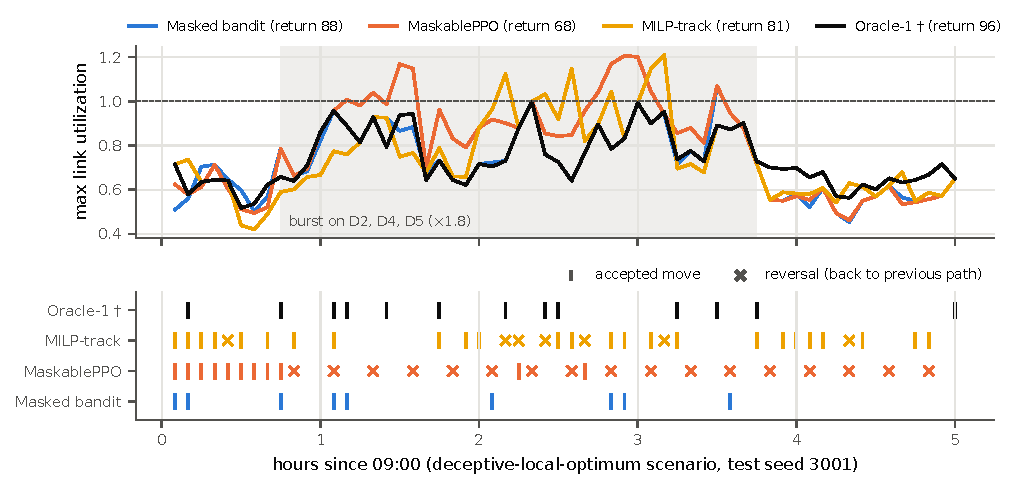
\includegraphics[width=\textwidth]{fig_case}
\caption{One test episode (deceptive-local-optimum, seed 3001; learners of root
314159). Top: worst link utilization; bottom: accepted moves ($\times$ = return to
the previous path within six intervals). PPO flips one demand every three
intervals, the hold-down period; the bandit makes few moves. Oracle-1 sees the
next interval's traffic and is shown for reference.}
\label{fig:case}
\end{figure*}

\section{Additional results}
\label{app:results}

\begin{table}[h]
\centering\small
\caption{Primary comparison per training root (mean test return over 140
episodes): selected checkpoint (validation seeds) and final 400k checkpoint.}
\label{tab:perroot}
\begin{tabular}{@{}rrrrrrr@{}}
\toprule
 & \multicolumn{3}{c}{Masked bandit} & \multicolumn{3}{c}{MaskablePPO} \\
\cmidrule(lr){2-4}\cmidrule(l){5-7}
Root & Selected & Return & Final & Selected & Return & Final \\
\midrule
\tabinput{tables/main_per_root}
\bottomrule
\end{tabular}
\end{table}

\begin{table}[h]
\centering\small
\caption{Learner minus reference, paired test returns (two-stage bootstrap 95\,\%
CI over roots and episodes) and the number of roots on which the difference is
positive.}
\label{tab:vsref}
\begin{tabular}{@{}llrr@{}}
\toprule
Learner & Reference & Difference [95\,\% CI] & Roots $>0$ \\
\midrule
\tabinput{tables/learners_vs_references}
\bottomrule
\end{tabular}
\end{table}

\begin{table}[h]
\centering\small
\caption{Sequentiality diagnostic per scenario at $H=24$ (states with at least 24
remaining intervals): agreement of the myopic and the 24-interval best action,
share of the 24-interval gain captured by the myopic action, and share of states
in which the 24-interval best action has negative immediate advantage, under
clairvoyant and frozen-exogenous rollouts (\%).}
\label{tab:seqscen}
\begin{tabular}{@{}lrrrrrrr@{}}
\toprule
 & & \multicolumn{3}{c}{Clairvoyant} & \multicolumn{3}{c}{Frozen exogenous} \\
\cmidrule(lr){3-5}\cmidrule(l){6-8}
Scenario & States & Agree & Captured & Sacrifice & Agree & Captured & Sacrifice \\
\midrule
\tabinput{tables/seqdiag_per_scenario}
\bottomrule
\end{tabular}
\end{table}

\begin{table}[h]
\centering\small
\caption{Inference cost per decision (process CPU time, one thread, 60 states of
a test episode) and training cost (400k transitions, wall time and throughput
measured with 3--6 concurrent jobs on 4 cores; the simulator dominates).}
\label{tab:compute}
\begin{tabular}{@{}lrrrrr@{}}
\toprule
Policy & Parameters & Train (min) & Transitions/s & ms / decision & p95 ms \\
\midrule
\tabinput{tables/compute}
\bottomrule
\end{tabular}
\end{table}


\chapter{Engineering, validation and reproduction}
\section{Governance and integrity checks}
Every V2 run is wrapped by \texttt{AuditedV2Env}, which rejects any action that
is illegal under the authoritative pre-action mask, checks that the post-step
mask in \texttt{info} equals a fresh mask, checks that the twelve reward
components sum bit-for-bit to the scalar reward, checks finiteness and flow
solver convergence, and re-verifies the protected-class projection of every
protected move. Each check aborts the run on failure; consequently the
historical ``zero failures'' counters only certify that runs completed. We
therefore audited the mask independently (Section~\ref{sec:maskaudit}).

The sixteen files that define the V2 problem are pinned to a signed-off commit
and compared byte-for-byte (line-ending canonicalized) before governed
training; the ordered candidate-path table is part of every checkpoint's
identity, because V2 reuses V1's action numbering with different paths.

\section{Action-mask audit}
\label{sec:maskaudit}
\begin{center}\small\begin{tabular}{@{}lr@{}}\toprule
states & 15,480 \\
actions checked & 1,068,120 \\
legal te actions & 711,848 \\
ppo states checked & 15,480 \\
protected legal moves & 155,408 \\
transitions & 15,480 \\
accepted moves & 7,832 \\
frr changes & 146 \\
states with failed link & 804 \\
states with disconnected demand & 144 \\
\midrule
violation: noop illegal & 0 \\
violation: decode mismatch & 0 \\
violation: mask validator disagreement & 0 \\
violation: masked action accepted & 0 \\
violation: masked action side effect & 0 \\
violation: legal action rejected & 0 \\
violation: legal action wrong path & 0 \\
violation: legal action no dwell & 0 \\
violation: protected projection violation & 0 \\
violation: legal over failed link & 0 \\
violation: mask not idempotent & 0 \\
violation: independent projection violation & 0 \\
violation: independent projection mismatch & 0 \\
violation: ppo illegal probability mass & 0 \\
\bottomrule\end{tabular}\end{center}


\section{Equivalence and reproduction tests}
\begin{itemize}
\item The study evaluator (\texttt{mplssim/study/episode.py}) reproduces the
governed evaluator's episode summaries exactly (unit test).
\item The study trainer reproduces the governed trainer's network parameters
bit for bit after 8{,}192 transitions for both learners (slow test).
\item The $\gamma=0$ Q-learner is bit-identical to the bandit; the $L=0$ delayed
variant is bit-identical to the frozen environment (unit tests).
\item All 21 baseline (policy, scenario) holdout cells of the closed study
reproduce to within $3\cdot10^{-14}$ on different hardware and operating system.
\end{itemize}


\chapter{Discussion and limitations}
\section{Discussion}
\label{sec:discussion}

\paragraph{What the results mean.} In this formulation the current LSP
assignment is genuine state, and a move constrains the future through
hold-downs, reversal costs and coupled protected-class legality. Yet a learner
that ignores the future reaches the return of a per-interval optimizer, and a
learner trained with an effective horizon of about 200 intervals
($1/(1-\gamma)$, 17 hours) does worse than both. The closed-loop oracle ladder
shows why there is little to gain from looking ahead: even with perfect
foresight, a controller that re-plans every interval gains only a few points
from lookahead beyond the next interval. When a move's effect is felt in the
interval in which it is made, the immediate reward ranks moves almost as a
longer criterion would; what is not myopic---anticipating bursts, failures
and diurnal change---is not provided by an observation without a clock or
forecasts. A sequential learner pays the price of a long-horizon objective
(noisy advantages, unstable optimization) without access to the signal that
would make it worthwhile.

\paragraph{Long horizons can hide small immediate costs.} The concrete failure
on three of five PPO roots is instructive for RL practice. Reconfiguration costs are small, immediate and
certain; congestion rewards are large, delayed and noisy. With $\gamma=0.995$
PPO's advantage estimates are dominated by the latter and fail to attribute
the former, so the policy settles into flipping a demand whenever the
hold-down allows. We have not measured the advantage noise directly. The
evidence for this explanation is that setting $\gamma=0$ removes the
oscillation and closes the gap; against it, the critic is not poorly fitted
in aggregate (explained variance at the last update
\PPOEVDefaultMin--\PPOEVDefaultMax{} with $\gamma=0.995$, versus
\PPOEVZeroMin--\PPOEVZeroMax{} with $\gamma=0$), so the failure would have to
lie in the small residual differences between moves rather than in the value
scale; and the PPO roots that do not oscillate fall short through lower network utility
rather than churn. The discount factor is thus a decisive hyper-parameter here, and the
default $\gamma\approx0.99$ that most RL-for-networking work inherits is not a
neutral choice when costs and benefits live on different time scales.

\paragraph{When is sequential RL justified?} Our evidence points to three
conditions, each testable before choosing an algorithm: (i) actions whose
effects are delayed relative to the decision, so that the immediate reward
does not contain them (\S\ref{sec:rq5}); (ii) exogenous dynamics that are
predictable from the observation, so that anticipation can be learned; and
(iii) decisions that change the future feasible set substantially. The
closed-loop oracle ladder of \S\ref{sec:sequentiality} bounds the value of
lookahead under perfect foresight and the frozen rollout measures how much
cost amortization changes the ranking of moves, both from a simulator without
learning; neither measures (iii) beyond the bound, because their continuation
never moves again. We recommend reporting both before choosing an algorithm.

\paragraph{When should simpler methods be preferred?} When effects are
immediate, a myopic learner---or, if a model of the objective is available, a
per-interval optimizer---reaches a higher return than PPO here. Inference cost
does not discriminate at a five-minute interval (the bandit needs
\InfBanditMs{}\,ms per decision, PPO \InfPPOMs{}\,ms, MILP-track
\InfMilpMs{}\,ms). The bandit and MILP-track trade differently: MILP-track
attains higher network utility and pays more in move costs, which its
objective does not contain; the bandit reroutes \ChurnRatioBanditMilp{} times
as often as MILP-track (\TestBanditReroutes{} vs.\ \TestMilpReroutes{} per
hour) at a return we cannot distinguish from MILP-track's, which matters
operationally because every LSP move is signalling and risk. A churn-aware
optimizer would be the natural stronger baseline.

\paragraph{Networking implications.} Teal and DOTE treat TE as a one-shot
problem per traffic matrix. Our results support that treatment in a setting
with persistent state, incremental changes and stability timers, where one
might have expected sequential structure to matter---as long as a change takes
effect within the interval in which it is decided, and in a heavily loaded
regime where TE mostly decides which traffic to lose (\S\ref{sec:limitations}). They also show that churn
metrics (reroutes, reversals) must be reported with the objective: PPO's best
root reaches a higher network utility than any bandit root (\PPOUtilMax{}
vs.\ at most \BanditUtilMax) but would be unacceptable to an operator because of its oscillation.

\paragraph{Generalization.} We make no claim beyond this simulator. Larger
topologies, elastic traffic, real traffic matrices and control-plane latency
all plausibly increase temporal coupling; the diagnostic and the
delayed-effect experiment indicate how to test that.

\section{Limitations}
\label{sec:limitations}

\paragraph{Simulator realism.} The model is flow-level: delay and loss are
analytic functions of utilization, traffic is exogenous and inelastic, the
control plane acts instantaneously, fast reroute is free, and telemetry is
exact. Learned routing policies trained in fluid models are known not to
transfer to packet-level dynamics~\citep{boltres2024packerl}; our conclusions
are about this model. Inelastic traffic in particular removes a natural
source of temporal coupling (congestion that suppresses future demand).

\paragraph{Formulation.} One trunk may move per interval network-wide and each
demand has four fixed candidate paths. These choices create the incremental,
stateful character of the problem; a controller that re-optimizes all trunks
at once faces the one-shot problem studied by Teal and DOTE instead. We did
not vary the number of candidates or the per-interval move limit, because the
environment definition is frozen.

\paragraph{Scale and data.} One hand-designed 18-router topology, 17 demands,
hand-written diurnal profiles and seven scripted test scenarios; no operator
traffic matrices or failure traces. No claim of topology generalization is
made.

\paragraph{Learning.} Five training roots for the primary comparison and
two to three for ablations; root-level intervals are wide and are reported.
A budget of 400k transitions (about 1{,}390 simulated days), with one longer
run per learner. PPO received a bounded one-factor sensitivity study, the
bandit none; neither used graph-structured networks, observation
normalization or learning-rate schedules. A discount below the true one can
help with limited data~\citep{jiang2015horizon,amit2020discount}, so ``the
myopic learner wins at this budget'' does not imply that no sequential
structure exists---which is why we measure the structure separately.

\paragraph{Objective.} All rankings use one hand-weighted operational reward;
we report its components and operational metrics alongside, but a different
operator objective could reorder close methods.

\paragraph{References.} The clairvoyant oracles see future traffic and only
evaluate ``one move, then no change''; they bound $H$-step-greedy reasoning, not
the optimal policy. MILP-track optimizes gross maximum utilization only.

\paragraph{Provenance.} The closed study's checkpoints and per-episode
holdout data were not archived; its learner results are compared at the
aggregate level it committed.


\chapter{Process record: failures and design history}
\section{From Environment V1 to V2}
The repository's first version (V1, branch \texttt{main}) trained a single
MaskablePPO agent (400k transitions, one seed) on a 586-feature observation and
a reward whose terms were mostly clipped. The V2 audit recorded in the code
(\texttt{mplssim/rl/reward\_v2.py}, \texttt{mplssim/sim/engine\_v2.py}) found
that over 13{,}200 audited V1 intervals the maximum-utilization term was
saturated 60.2\,\% of the time, loss 41.1\,\% and delay 26.2\,\%, so a link at
400\,\% utilization scored like one at 100\,\%; that congestion and SLA failures
were counted twice; and that a flat 0.08 reroute price was repaid by a
0.027 reduction in utilization. The published V1 PPO policy consequently made
an accepted TE move in all 3{,}300 evaluation intervals, 91.7\,\% of them
reversals on \texttt{full\_day}. V1 also processed link events one tick late
(a controller could act on a topology it was told was healthy), reused episode
seeds across workers (80 distinct collisions within 30 episodes), admitted two
candidate paths that transited provider-edge routers, and loaded every hop of
a path with the full offered demand even after upstream drops.

V2 fixed each of these: right-closed event windows, collision-free seeds,
role-valid candidates, a carried-flow fixed point, an unsaturated
severity-ordered utility, a bounded potential-shaping term and a move cost
proportional to what a move disturbs, plus a hard three-interval dwell. Its
definition was frozen and signed off (commit \texttt{dca533b}) before any V2
learner was trained. These V1 findings are historical (reported in code
documentation, not re-executed here).

\section{The closed V2 study}
The V2 study was run as a governed sequence: a seed-42 pilot, a three-root
continuity study, and a single untouched final holdout. Its own failures are
preserved in its reports: an SB3 seed-propagation bug that invalidated the
first PPO run (the wrapper now preserves the governed root and the run fails
closed on any other root), two governance repairs needed to admit the
preregistered roots, and a CUDA preflight failure before any holdout episode.

\section{Failures in this study}
{\small\begin{longtable}{@{}rp{0.5\textwidth}p{0.38\textwidth}@{}}\toprule
\# & Event & Outcome \\\midrule
1 & Full test suite on fresh install & 802 passed, 10 skipped, 16 failed; all failures = missing external checkpoints [process] \\
2 & 8,192-transition smoke runs of both governed learners (CPU) & ok; 155--157 transitions/s single-process \\
3 & First launch of 6 governed reproduction runs in the main checkout & \textbf{all 6 aborted at start}: governed trainer refuses a dirty checkout (an untracked \texttt{logs/\allowbreak{}} directory) [process]. Relaunched in a clean detached worktree at \texttt{1457e9b} (\texttt{.\allowbreak{}worktrees/\allowbreak{}repro}). \\
4 & Relaunch: roots 42, 314159 (PPO), 42 (bandit) first, 3 in parallel & running \\
5 & Sequentiality diagnostic, greedy reference, seeds 4001--4003, H $\le$ 24, clairvoyant & see \texttt{docs/\allowbreak{}SEQUENTIALITY\_\allowbreak{}AUDIT.\allowbreak{}md} \\
6 & \texttt{scripts/\allowbreak{}study/\allowbreak{}queue.\allowbreak{}py} crashed on import: module name shadowed stdlib \texttt{queue} (imported by networkx) [process] & renamed to \texttt{scheduler.\allowbreak{}py} \\
7 & Study-trainer equivalence test (8,192 transitions, both learners) & \textbf{bit-identical} network parameters to the governed trainer \\
8 & Baselines on historical holdout seeds 1001--1005 & all 21 (policy, scenario) means reproduce historical values to $\le$ 3e-14 \\
9 & Mask audit pass 1 (engine-side checks) & 15,480 states, 1,068,120 checks, 0 violations \\
10 & Early look at diagnostic (full\_day): myopic action agrees with 24-step best in 35 \% of states. Added frozen-exogenous counterfactual to separate predictable persistence value from clairvoyant anticipation. & frozen run queued after \#5 \\
11 & Mask audit pass 2 (+ independent from-scratch projection, + PPO probability mass) & see \texttt{docs/\allowbreak{}MASK\_\allowbreak{}VALIDATION.\allowbreak{}md} \\
12 & Diagnostics launched with \texttt{nice} still took ~75 \% of CPU: kernel autogroup scheduling ignores niceness across sessions [process] & disabled \texttt{kernel.\allowbreak{}sched\_\allowbreak{}autogroup\_\allowbreak{}enabled}; training throughput restored \\
13 & First reproduction trio finished (bandit r42, PPO r42, PPO r314159); second trio started & evaluated automatically under both protocols \\
14 & Study scheduler had never started (it counted the four low-priority diagnostics as occupying slots); on restart it launched 3 jobs because it matched only commands starting with \texttt{python} and not \texttt{/\allowbreak{}usr/\allowbreak{}bin/\allowbreak{}python} [process] & fixed process matching; scheduler now also skips runs already executing (a restart would otherwise have renamed a live run directory) \\
15 & All 6 reproductions evaluated; E1 bandit r161803, r141421 and PPO r161803 completed & \texttt{docs/\allowbreak{}REPRODUCTION\_\allowbreak{}REPORT.\allowbreak{}md} \\
16 & \textbf{Worker restart killed every background process} [process]. Lost: E1 PPO r141421 (608 episodes) and E2 qg05 r42 (672 episodes) mid-training, mask-audit pass 2, partial diagnostics. Persisted: all completed runs and every per-episode output. & interrupted run directories kept as \texttt{*.\allowbreak{}interrupted}; runs restarted from scratch (study checkpoints hold no replay buffer, so they are not resumable); diagnostics resumed per file; \texttt{scripts/\allowbreak{}study/\allowbreak{}relaunch\_\allowbreak{}background.\allowbreak{}sh} makes relaunch idempotent \\
17 & MILP-track on all 140 test episodes & statistically indistinguishable from the bandit; above PPO [science] \\
18 & Model fidelity (root 42) and deceptive-scenario case study & PPO's actions are worse than no-op over 6 intervals; PPO flips one demand every 3 intervals (hold-down expiry) [science] \\
19 & Return decomposition over all test episodes & on 3 of 4 PPO roots > 50 \% of moves are reversals; PPO's network utility is comparable to the bandit's but move/reversal costs are 5--13$\times$ larger; shaping contributes $\le$ 0.02 per episode [science] \\
20 & Frozen-exogenous sequentiality diagnostic complete (495 states paired with the clairvoyant pass) & myopic = 24-step best in 88 \% of states with traffic frozen vs 33 \% with true future; non-myopic value is anticipation of exogenous change [science]. Motivated post-hoc E7 (\texttt{docs/\allowbreak{}HYPOTHESES.\allowbreak{}md} H9) \\
21 & E1 complete (5 roots per learner) & bandit $-$ PPO positive on 5/5 roots \\
22 & E2 PPO $\gamma$ = 0, 3 roots & \textbf{23.6 vs bandit 24.2 on the same roots ($-$0.6 [$-$5.2, 2.7]); PPO $\gamma$ = 0.995: $-$6.4.} Flapping disappears ($\le$ 2.4 reversals/episode). Supports H2 and H10 [science] \\
23 & Compute re-planning ($\approx$34 run-equivalents left). Training slots 3 $\to$ 4; queue reordered by information value (Q $\gamma$0.9 $\to$ E4 $\to$ E7 $\to$ PPO $\gamma$0.9 $\to$ E3 $\to$ rest of E2 $\to$ E6 $\to$ E5). E3 trimmed from 8 to 6 configurations (\texttt{ns128}, \texttt{net64} dropped \textbf{before running}) [process] &  \\
24 & Oracle-3 complete (5 test seeds) & Oracle-3 $-$ Oracle-1 = +2.9 [1.5, 4.2], versus Oracle-1 $-$ bandit $\approx$ 22 on the same episodes [science] \\
25 & E2 Q-learner $\gamma$ = 0.9, 3 roots & 19.4 vs bandit 24.2 ($-$4.8 [$-$7.0, $-$2.1]), 0/3 roots better; supports H3 [science] \\
26 & E4 delayed activation (L = 1), bandit and PPO, roots 42/314159 & bandit 22.0 $\to$ $-$30.3; PPO 1.6 $\to$ 1.2; PPO $-$ bandit = +31.5 [20.6, 42.6] under delay, 2/2 roots. Supports H6 [science] \\
27 & Oracle-6 complete (5 test seeds) & Oracle-6 $-$ Oracle-1 = +1.4 [0.5, 2.5]; Oracle-1 $-$ bandit $\approx$ 22 [science] \\
28 & E3 extended (post-hoc, before any E3 result): \texttt{rewnorm} (reward normalization) and \texttt{gae08} (GAE $\lambda$ = 0.8), variance-reduction knobs that target the proposed mechanism while keeping $\gamma$ = 0.995 & queued \\
29 & \textbf{E3 selection rule fixed before any E3 result:} each configuration's score is the validation mean (seeds 2001--2005, 35 episodes) of its best checkpoint, exactly as checkpoint selection for every learner. The configuration with the highest score is retrained on roots 314159 and 271828 (E3b) if its score exceeds the default PPO's root-42 validation score; otherwise E3 is reported as "no configuration improved validation return" and E3b is not run. Test returns of E3 runs are reported for completeness only and play no role in selection. Caveat recorded in advance: one-root selection is noisy, given per-root shifts of up to 41 points from numerical noise alone (\#15) [process] &  \\
30 & Sequentiality diagnostic on the delayed variant (L = 1), frozen pass first, then clairvoyant; greedy reference, seeds 4001--4003. Post-hoc (H11), recorded before launch; tests whether the diagnostic flags the regime where the bandit fails [science] & running (low priority) \\
31 & \textbf{Correction to \#19} (written when 4 PPO roots were available): with all 5 roots, PPO's mean network utility is clearly below the bandit's (18.4 vs 28.0). The bandit $-$ PPO gap of 24.9 splits into 15.3 from move/reversal costs (61 \%) and 9.6 from utility; PPO's per-root utility ranges from 7.8 to 32.2. One root (161803) does not flap (0 \% reversals) but earns low utility. "Utility comparable to the bandit's" is withdrawn; costs remain the larger part of the gap [science] & paper \S{}5 and \texttt{docs/\allowbreak{}RESEARCH\_\allowbreak{}OVERVIEW.\allowbreak{}md} F3 updated \\
32 & Round-2 hostile review (\texttt{docs/\allowbreak{}HOSTILE\_\allowbreak{}REVIEWS.\allowbreak{}md}): MILP-track's two parameters were never tuned and it moves the largest-volume demand, which is the most expensive move under V2's volume-proportional cost. \textbf{MILP-track tuning on validation seeds} (2001--2005, all 7 scenarios): min\_gain $\in$ {0, 0.02, 0.05, 0.10} $\times$ move selection $\in$ {largest, smallest volume}; selection = highest validation mean; the selected configuration is then run on the 140 test episodes and reported next to the untuned default (which stays in every table) [science] & running \\
33 & Round-2 review N4: is the delay result "sequential RL is needed" or "regressing the decision-time reward fails"? Added \texttt{E4\_\allowbreak{}delay} tag \texttt{L1\_\allowbreak{}qg05} (Q-learner $\gamma$ = 0.5, effective horizon $\approx$ 2, roots 42/314159), post-hoc, before any result. If it recovers the no-delay return, a two-interval horizon suffices and "long-horizon RL is needed" would be an overclaim [science] & queued \\
34 & Round-2 review R5: rollouts with a no-change continuation cannot see value from later moves. Added a reactive continuation (fresh greedy controller after the first move; tested to equal real execution and to restore state exactly). Queued after the delayed diagnostic: frozen, then clairvoyant, greedy reference, seeds 4001--4003 (H12, recorded before launch) [science] & queued \\
35 & E2 PPO $\gamma$ = 0.9, 3 roots & 15.4 (above the bandit on 0/3 roots), between $\gamma$ = 0 (23.6) and $\gamma$ = 0.995 ($-$6.4): PPO's return falls monotonically with its horizon; close to Q $\gamma$ = 0.9 (19.4). Bears on round-2 R3: horizon, not a PPO-specific failure [science] \\
36 & E4 Q $\gamma$ = 0.5 under delay, 2 roots (\#33) & $-$2.0 under delay vs 24.6 without; above the bandit on 2/2 roots but below PPO (1.2) and far below MILP-track (11.3). A short bootstrapped horizon does not recover the delayed value at this budget [science] \\
37 & E7 time of day, 2 roots each & clock adds +1.9 to the bandit (2/2 roots) and +0.4 to Q $\gamma$ = 0.9 (1/2 roots). \textbf{H9 not supported}: the clock is used as context for the immediate reward, not for planning [science] \\
38 & \textbf{E3 selection} (rule \#29). Validation best-checkpoint means on root 42: ent003 15.3, gae08 13.7, rewnorm $-$5.1, lr1e4 $-$23.9, lr1e3 $-$24.7, ent0 $-$26.2, clip01 $-$27.8, ns2048 $-$28.2; default PPO $-$19.1; bandit 12.2. Selected: \textbf{ent\_coef = 0.03}. Its root-42 test return (20.7) exceeds the bandit's on the same root (18.3): \textbf{H4 is falsified on the selection root}. Root 42 is the default PPO's worst root, so E3b retrains ent003 on roots 314159/271828 (rule) and 161803/141421 (added now, before any E3b result) [science] & E3b queued first \\
40 & \textbf{E3b}: tuned PPO (ent 0.03) on the four fresh primary roots & selected-checkpoint test returns 12.9 / $-$10.1 / 6.1 / $-$15.8 (roots 314159 / 271828 / 161803 / 141421) vs bandit 25.8 / 28.4 / 28.5 / 25.0 and default PPO 16.9 / $-$22.5 / 5.8 / 14.8. Tuned PPO is below the bandit on \textbf{4/4} fresh roots and not better than default PPO on average; two roots still flap (43--58 reversals/episode). The root-42 improvement (\#38) did not transfer: \textbf{H4 supported on fresh roots} [science] \\
41 & E2 Q-learner $\gamma$ = 0.99, 3 roots & 3.3 ($-$20.9 vs the bandit; 0/3 roots better). Return falls with the discount in the value family as in PPO; \textbf{H3 supported} [science] \\
42 & E6 bandit without shaping, root 42 (root 314159 pending) & 26.7 vs 18.3 with shaping (+8.4): shaping does not help the bandit on this root [science] \\
44 & Tuned MILP-track (min\_gain 0.10, largest) on the 140 test episodes & \textbf{30.9 [28.8, 33.0]}, 3.77 reroutes/h; bandit $-$ tuned MILP = $-$5.7 (t-interval [$-$10.9, $-$0.5]; bandit ahead on 0/5 roots); PPO $-$ tuned MILP = $-$30.6. With two parameters chosen on validation seeds, per-interval optimization beats both learners. The "bandit matches the optimizer" statement now holds only for the untuned default [science] \\
45 & E6 bandit without shaping, both roots & +8.4 / +5.4 (28.9 vs 22.0): the shaping term costs the bandit return; its advantage over PPO does not rest on shaping [science] \\
46 & Round-3 hostile review (\texttt{docs/\allowbreak{}HOSTILE\_\allowbreak{}REVIEWS.\allowbreak{}md}): shaping confounds the horizon sweep (R-b); no within-root noise floor (R-c). Registered \textbf{E6b} (Q $\gamma$ = 0.9, PPO $\gamma$ = 0, PPO $\gamma$ = 0.995, all without shaping, roots 42/314159; H13) and \textbf{E8} (default bandit, root 42, learner seeds 9001/9002, identical traffic; H14), before any result. Trainer: new optional \texttt{learner\_\allowbreak{}seed} override (default = root, so all earlier runs are unchanged) [science] & queued \\
47 & \textbf{E8} learner-seed noise floor (bandit, root 42, identical traffic) & test returns 18.3 (original) / 17.8 / 28.2: a \textbf{10-point spread from the learner seed alone. H14 falsified.} E6 (+8.4 / +5.4), E7 (+1.9 / +0.4), Q $\gamma$ = 0.5 (+1.4) and the root-42 tuned-PPO win (+2.4) are within learner noise and are now reported as inconclusive. The 5-root main comparison is unaffected (its t-interval is over roots, each varying the learner seed too). The reproduction contrast (PPO shifts up to 41, bandit up to 4) is qualified: the bandit is less sensitive, not insensitive [science] \\
48 & \textbf{E6b} horizon contrasts without shaping (roots 42 / 314159), minus the shaping-free bandit (26.7 / 31.2) & PPO $\gamma$ = 0: 25.4 / 24.0 ($-$1.3 / $-$7.2); Q $\gamma$ = 0.9: 13.1 / 15.8 ($-$13.6 / $-$15.4); PPO $\gamma$ = 0.995: $-$19.4 / 14.9 ($-$46.1 / $-$16.3; root 42 flaps with 74 reversals per episode). The ordering of the shaped sweep holds on both roots: \textbf{H13 supported}; the horizon effect is not a shaping artifact [science] \\
\bottomrule\end{longtable}}



\chapter{Conclusion}
\section{Conclusion}
\label{sec:conclusion}

For an incremental, masked MPLS traffic-engineering problem with persistent
routing state, a masked contextual bandit beats MaskablePPO on every training
root and matches a per-interval MILP optimizer. The cause is the planning
horizon, not the learning algorithm: PPO with $\gamma=0$ matches the bandit,
while PPO with $\gamma=0.995$ settles into costly oscillations, and a
bootstrapped value learner does not improve on the bandit. A sequentiality
diagnostic shows why: almost all of the problem's non-myopic value lies in
anticipating exogenous change that the controller cannot observe, while the
predictable part is captured by the first interval's reward. Sequential RL
should therefore be justified by measured temporal coupling---delayed effects
or predictable dynamics---rather than assumed from the fact that the problem
is formally an MDP.


\bibliographystyle{plainnat}
\bibliography{../paper/references}
\end{document}
